	\section{Onsager inequality} \label{inequality}
We show that the active nematic system evolves in a way that the proposed dissipation potential is always positive, that is, 
\begin{align}
	d &  = \eta \big( d_{ab} d_{ab}   + (\text{tr}d)^2  \big) + \frac{\eta_{\text{rot}}}{2} \widehat{q}_{ab} \widehat{q}_{ab}  + \beta d_{ab}^{\rm dev}\widehat{q}_{ab} + \frac{\gamma}{2} v_a v_a \geq 0  \\ & = 
	2\eta \big( d_{11}^2 + d_{12}^2 + d_{22}^2  + d_{11}d_{22} \big) + \eta_{\text{rot}} \big( \widehat{q}_{1}^{\, \, 2} + \widehat{q}_{2}^{\, \, 2}  \big) + \beta \big(d_{11}\widehat{q}_{1} - d_{22}\widehat{q}_{1} + \nonumber  2d_{12}\widehat{q}_{2}\big)  \\ &  +  \nonumber  \frac{\gamma}{2} \big(v_1^{\,2} + v_2^{\,2}\big) \geq 0 \nonumber.
\end{align}
In form of matrix, the component-wise dissipation potential is re-written as $	z_{a} M_{ab} z_b\geq 0,$
where
\begin{align}
	\bm{z} = \begin{pmatrix}
		d_{11}\\ 
		d_{22}\\ 
		d_{12}\\ 
		q_{1}\\ 
		q_{2}\\ 
		v_1\\ 
		v_2\\ 
	\end{pmatrix}, \quad  \bm{M} = \begin{pmatrix}
		2\eta& \eta &0  &\beta/2  &0  &0  &0   \\ 
		\eta& 2\eta &0  &-\beta/2  &0  &0  &0   \\ 
		0&  0&  2\eta&  0& \beta &0  &0   \\ 
		\beta/2& -\beta/2 &0  &\eta_{\rm rot}  &0  &0  &0   \\ 
		0&  0 &\beta  & 0 & \eta_{\rm rot} &0  &0   \\ 
		0& 0 & 0 & 0 & 0 & \gamma/2 & 0  \\ 
		0& 0 & 0 & 0 & 0 & 0 & \gamma/2
	\end{pmatrix}.
\end{align}
According to the Sylvester's criterion \cite{doi:10.1080/00029890.1991.11995702}, for $\bm{M}$ to be a positive definite tensor it should be symmetric with positive leading principal minors. Upon inspecting the principle minors of matrix $\bm{M}$, we arrive to the following condition on the model parameters that ensures that $ d  \geq 0$
\begin{equation}
	2\eta \eta_{\rm rot} - \beta^2 \geq 0.
\end{equation}
\section{Equivalence between weak and strong forms} \label{equivalence}

In this section, we establish an equivalence between strong and weak balance of force conjugate to velocities. For doing so, we have to prove that
\begin{equation}
	\label{eq:weak_v_disc_app}
	\begin{aligned}
		&\underset{ A}{\int} \bigg \{-\frac{ f}{\rho} \nabla_d \left(\rho u_d\right)  + \frac{\partial ( d+ p)}{\partial \widehat{q}_{ab}}  \left[\nabla_c q_{ab} u_c +\frac{1}{2}\left(q_{ac} \epsilon_{cb}-\epsilon_{ac}q_{cb}\right) \epsilon_{de}\nabla_e u_d\right] \bigg \}\rho dA \\
		&+  \int_{\partial_{N_{\bm{t}}} A} \bigg\{f\rho N_c u_c - L_{ab} \left[\nabla_c q_{ab} u_c +\frac{1}{2}\left(q_{ac} \epsilon_{cb}-\epsilon_{ac}q_{cb}\right) \epsilon_{de}\nabla_e u_d\right] \bigg\}dl,
	\end{aligned}
\end{equation}
is equal to 
\begin{equation}
	\label{eq:weak_v_app}
	\begin{aligned}
		\underset{A}{\int} \sigma^e_{ab}\nabla_b u_a dA + \int_{\partial_{N_{\bm{t}}} A} ( m_c N_c)\epsilon_{ab} \nabla_b v_a dl,
	\end{aligned}
\end{equation}
where $\bm{\sigma}^e$ is the elastic part of the total stress, i.e, 
\begin{equation}
	\sigma_{ab}^e = -\frac{1}{2} \bigg[\left(\nabla\cdot\bm{m}\right)\epsilon_{ab} - \rho \left(\frac{\partial  f}{\partial \nabla_b q_{dc}} \nabla_a q_{dc}+ \frac{\partial  f}{\partial \nabla_a q_{dc}} \nabla_b q_{dc}\right) \bigg].
\end{equation}
We first integrate the first term in the second line of Eq.~\eqref{eq:weak_v_disc_app}, to get
\begin{equation}
	\label{eq:weak_v_disc_app2}
	\begin{aligned}
		&\underset{ A}{\int} \bigg \{  u_d \nabla_d f + \frac{\partial ( d+ p)}{\partial \widehat{q}_{ab}} \left[\nabla_c q_{ab} u_c +\frac{1}{2}\left(q_{ac} \epsilon_{cb}-\epsilon_{ac}q_{cb}\right) \epsilon_{de}\nabla_e u_d\right] \bigg \} \rho dA \\
		&+  \int_{\partial_{N_{\bm{t}}} A} \bigg\{ -L_{ab} \left[\nabla_c q_{ab} u_c +\frac{1}{2}\left(q_{ac} \epsilon_{cb}-\epsilon_{ac}q_{cb}\right) \epsilon_{de}\nabla_e u_d\right]  \bigg\}dl.
	\end{aligned}
\end{equation}
We now note that from the first expression in Eq.~\eqref{eq:balance_q}
\begin{equation}
	\frac{\partial ( d+ p)}{\partial \widehat{q}_{ab}} =  \frac{1}{\rho}\nabla_c \left(\rho \frac{\partial f}{\partial \nabla_c q_{ab}} \right) - \frac{\partial f}{\partial q_{ab}}, 
\end{equation}
and thus
\begin{equation}
	\label{eq:weak_v_disc_app3}
	\begin{aligned}
		&\underset{ A}{\int} \bigg \{  u_d \nabla_d f + \left[ \frac{1}{\rho}\nabla_c \left(\rho \frac{\partial f}{\partial \nabla_c q_{ab}}\right) - \frac{\partial f}{\partial q_{ab}} \right] \left[\nabla_c q_{ab} u_c +\frac{1}{2}\left(q_{ac} \epsilon_{cb}-\epsilon_{ac}q_{cb}\right) \epsilon_{de}\nabla_e u_d\right] \bigg \} \rho dA \\
		&+  \int_{\partial_{N_{\bm{t}}} A} \bigg\{  -L_{ab} \left[\nabla_c q_{ab} u_c +\frac{1}{2}\left(q_{ac} \epsilon_{cb}-\epsilon_{ac}q_{cb}\right) \epsilon_{de}\nabla_e u_d\right]  \bigg\}dl.
	\end{aligned}
\end{equation}
We integrate by parts the first term in the first square brackets 
\begin{equation}
	\label{eq:weak_v_disc_app4}
	\begin{aligned}
		&\underset{ A}{\int} \bigg \{  u_d \nabla_d f - \frac{\partial f}{\partial q_{ab}} \left[\nabla_c q_{ab} u_c +\frac{1}{2}\left(q_{ac} \epsilon_{cb}-\epsilon_{ac}q_{cb}\right) \epsilon_{de}\nabla_e u_d\right] \\
		&- \left( \frac{\partial f}{\partial \nabla_c q_{ab}}\right) \nabla_c \left[\nabla_d q_{ab} u_d +\frac{1}{2}\left(q_{ad} \epsilon_{db}-\epsilon_{ad}q_{db}\right) \epsilon_{ef}\nabla_f u_e\right] \bigg \} \rho dA \\
		&+  \int_{\partial_{N_{\bm{t}}} A} \bigg\{ \left[\left(\rho \frac{\partial f}{\partial \nabla_c q_{ab}}\right) N_c-L_{ab} \right] \left[\nabla_c q_{ab} u_c +\frac{1}{2}\left(q_{ac} \epsilon_{cb}-\epsilon_{ac}q_{cb}\right) \epsilon_{de}\nabla_e u_d\right]   \bigg\}dl,
	\end{aligned}
\end{equation}
but the first term in the boundary cancels because of the second line of Eq.~\eqref{eq:balance_q}, so we have
\begin{equation}
	\begin{aligned}
		&\underset{ A}{\int} \bigg \{  u_d \nabla_d f - \frac{\partial f}{\partial q_{ab}} \left[\nabla_c q_{ab} u_c +\frac{1}{2}\left(q_{ac} \epsilon_{cb}-\epsilon_{ac}q_{cb}\right) \epsilon_{de}\nabla_e u_d\right] \\
		&- \left( \frac{\partial f}{\partial \nabla_c q_{ab}}\right) \nabla_c \bigg[\nabla_d q_{ab} u_d +\frac{1}{2}\left(q_{ad} \epsilon_{db}-\epsilon_{ad}q_{db}\right) \epsilon_{ef}\nabla_f u_e\bigg] \bigg \} \rho dA.
	\end{aligned}
\end{equation}
Furthermore, we now note that 
\begin{equation}
	\nabla_d f = \frac{\partial f}{\partial q_{ab}}\nabla_d q_{ab} + \frac{\partial f}{\partial \nabla_c q_{ab}} \nabla_c \nabla_d q_{ab}.
\end{equation}
After plugging the expression above in Eq.~(\ref{eq:weak_v_disc_app4}), we simplify the expression above to 
\begin{equation}
	\label{eq:weak_v_disc_app5}
	\begin{aligned}
		&\underset{ A}{\int} \bigg \{   - \frac{\partial f}{\partial q_{ab}}  \bigg[\frac{1}{2}\left(q_{ac} \epsilon_{cb}-\epsilon_{ac}q_{cb}\right) \epsilon_{de}\nabla_e u_d\bigg] \\
		&-  \frac{\partial f}{\partial \nabla_c q_{ab}} \nabla_d q_{ab} \nabla_c u_d + \frac{1}{2} \frac{\partial f}{\partial \nabla_c q_{ab}} \nabla_c\bigg[\left(q_{ad} \epsilon_{db}-\epsilon_{ad}q_{db}\right) \epsilon_{ef}\nabla_f u_e\bigg] \bigg \} \rho dA .
	\end{aligned}
\end{equation}
Due to the symmetry to $q_{ab}$ the first term above is rendered zero and the expression is simplified to
\begin{equation}
	\label{eq:weak_v_disc_app6}
	\begin{aligned}
		&\underset{ A}{\int} \bigg \{ -\frac{\partial f}{\partial \nabla_c q_{ab}}  \nabla_d q_{ab} \nabla_c u_d +\frac{1}{2} \frac{\partial f}{\partial \nabla_c q_{ab}} \nabla_c\bigg[\left(q_{ad} \epsilon_{db}-\epsilon_{ad}q_{db}\right) \epsilon_{ef}\nabla_f u_e\bigg] \bigg \} \rho dA ,
	\end{aligned}
\end{equation}
We symmetrize the first term above as
\begin{equation}
	\label{eq:weak_v_disc_app7}
	\begin{aligned}
		&\underset{ A}{\int} \frac{1}{2}\bigg \{  -\left(\frac{\partial f}{\partial \nabla_c q_{ab}}  \nabla_d q_{ab} + \frac{\partial f}{\partial \nabla_d q_{ab}}  \nabla_c q_{ab}  \right)\nabla_c u_d + \frac{\partial f}{\partial \nabla_c q_{ab}} \nabla_c\bigg[\left(q_{ad} \epsilon_{db}-\epsilon_{ad}q_{db}\right) \epsilon_{ef}\nabla_f u_e\bigg] \bigg \} \rho dA ,
	\end{aligned}
\end{equation}
Now we apply integration by parts to term in the square bracket above and apply the divergence theorem
\begin{equation}
	\label{eq:weak_v_disc_app8}
	\begin{aligned}
		&\underset{ A}{\int} \frac{1}{2}\bigg \{  -\left(\frac{\partial f}{\partial \nabla_c q_{ab}}  \nabla_d q_{ab} + \frac{\partial f}{\partial \nabla_d q_{ab}}  \nabla_c q_{ab}  \right)\nabla_c u_d - \nabla_c \left( \frac{\partial f}{\partial \nabla_c q_{ab}}\right)  \left(q_{ad} \epsilon_{db}-\epsilon_{ad}q_{db}\right) \epsilon_{ef}\nabla_f u_e \bigg \} \rho dA   \\
		& + \underset{ \partial A}{\int} \frac{1}{2}\frac{\partial f}{\partial \nabla_c q_{ab}} \left(q_{ad} \epsilon_{db}-\epsilon_{ad}q_{db} \right) \epsilon_{ef} N_c \nabla_f u_e \rho d l .
	\end{aligned}
\end{equation}
Finally, by taking into account Eqs.~\eqref{eq:sym_stress}, \eqref{eq:moment}, and \eqref{eq:balance_angular_momentum}, one can write the expression above as in Eq.~\eqref{eq:weak_v_app}.
\section{Grid convergence analysis} \label{appendix_grid}
We validate our numerical methods for the spatial discretization by solving the proposed model for various mesh sizes. For this purpose, we use a test case of a passive nematic system in circular confinements, see Fig.~\ref{sec_1_chap_3_fig_2}, for $\ell_p/\ell_0=0.04$. We use the normalized error of free-energy at steady state 
\begin{align}	
	e^x = \frac{|F^h -F^*|}{|F^*|} , 
\end{align}
where $F^h$ is the free-energy of a finite element solution with mesh-size $h$ and $F^*$ is that of an overkill solution computed with a very fine mesh of $n_e = 695,296$ triangular elements. We plot the energy error norm for decreasing mesh sizes, Fig.~\ref{grid}(a). The results show the expected optimal convergence (slope of 2 in a log-log scale) for linear elements. 


Next for the same numerical experiment, we validate the temporal convergence by gradually decreasing the
time step $\Delta t$ used to reach a fixed time point $t|a|/\eta_{\rm rot}=1$. We calculate the relative  the error norm  as
\begin{align}	
	e^t = \frac{|F^{\Delta t} -F^{t,*}|}{|F^{t,*}|} , 
\end{align}
where $F^{\Delta t}$ is the free-energy obtained with time-step $\Delta t$  at $t|a|/\eta_{\rm rot}=1$ and   $F^{t,*}$ is the free-energy with a very small time-step $\Delta t^* = 10^{-5}$. As expected, Fig.~\ref{grid}(b), the free-energy converges with a slope $\sim \Delta t$.
\begin{figure}[tb]
	\centering
	\includegraphics[width=\textwidth]{append.pdf}
	\caption{\label{grid} Validation of convergence behaviour of the numerical model. (a) Convergence of the spatial discretisation. The relative free-energy error $e^x$  shows a convergence rate $\sim h^{2}$. (b) Convergence of the temporal discretisation. The relative free-energy error  $e^{\Delta t}$  shows a convergence rate $\sim \Delta t$.}
\end{figure}

	\section{\label{sec:level1}1D reduced model} \label{appendix_1_sec_4}

To perform the linear stability analysis, we reduce the theoretical model to 1D  by considering the flow velocity $v(x,t)$  and the density field as $\rho(x,t)$ along the $x-$axis. The nematic order tensor is defined as $q_{ij} = S(n_i n_j - \delta_{ij}/2)$, where $\bm{n}$ is the local average filament orientation and $S$ is the local degree of alignment. Since it is traceless and symmetric, in general it can be represented by 2 independent degrees of freedom, $q_{11}=-q_{22}=q_1$ and $q_{12}=q_{21}=q_2$. In the 1D model we assume that $\bm{n}$ is either along or perpendicular to $x$, and hence $q_{12}=q_{21}=0$. We are thus left with one independent degree of freedom $q_{11}=-q_{22}=q$. Positive (negative) $q$ represents alignment along (perpendicular to) the $x-$axis. The Jaumann derivative of the nematic order parameter reduces in 1D to
\begin{equation}
	\hat{q}=\frac{\partial q}{\partial t} + v \frac{\partial q}{\partial x}.
\end{equation}
Particularizing the general equations given in the Chapter~\ref{chap_4} and systematically derived in Chapter~\ref{chap_2}, we present next the 1D governing equations pertinent to the linear stability analysis. Mass conservation reads
\begin{equation} \label{eq_1D_thick}
	\frac{\partial \rho }{\partial t}  + \frac{\partial}{\partial x} \left( \rho v \right)   -  D \frac{\partial^2 \rho}{\partial x^2}  + k_d (\rho-\rho_0)=0,
\end{equation}
balance of linear momentum of the active gel reduces to
\begin{equation} \label{eq_1D_force_balance}
	\rho \gamma   v =    \frac{\partial \sigma}{\partial x}   \, ,
\end{equation}
where stress along $x$, $\sigma$, is given by
\begin{equation} \label{eq_1D_stress}
	\sigma = \rho \left[  4 \eta \frac{\partial v}{\partial x}+ \beta  \hat{q}  +  \lambda \left( 1+\kappa q \right) - 2L \left( \frac{\partial q}{\partial x}\right)^2  \right].
\end{equation}
The evolution of nematic order $q$ is governed in the 1D setting by
\begin{equation} \label{eq_1D_torque}
	\eta_{\text{rot}} \hat{q} + \frac{\beta}{2} \frac{\partial v}{\partial x}+\left(2a - \rho \lambda_{\odot}+ 4bq^2\right)q - L \frac{\partial^2 \, q}{\partial x^2} - \frac{L}{\rho} \frac{\partial \, q}{\partial x} \frac{\partial \, \rho}{\partial x} = 0 \, .
\end{equation}
For $c_0=2a-\rho_0 \lambda_{\odot} \ge 0$, the uniform steady state of the system is given by $\rho(x,t) = \rho_0$, $v(x,t)=0$ and $q(x,t) = 0$. For $c_0<0$, the uniform steady state has spontaneous alignment given by  $q(x,t) = q_0 = \pm \frac{1}{2} \sqrt{-c_0/b}$. Finally, we note that, for the dissipation to be positive, the material parameters need to satisfy Onsager's inequality $4\eta \eta_{\rm rot} - \beta^2 \ge 0$ in the reduced one-dimensional model and  $2\eta \eta_{\rm rot} - \beta^2 \ge 0$ in the two-dimensional model, see Section~\ref{inequality}.

\pagebreak
\section{\label{sec:level2}Non-dimensionalization}  \label{appendix_1_sec_5}


We present next a non-dimensionalization of the governing Eqs.~(\ref{eq_1D_thick}$-$\ref{eq_1D_torque}). We choose the hydrodynamical length-scale $\ell_s=\sqrt{\eta / \gamma}$, above (below) which friction (viscosity) is the dominant dissipative mechanism in the active gel, and the time-scale of diffusion over this length-scale, $t_0 = \ell_s^2  /  D = \eta /(\gamma D)$. Using these characteristic scales, we non-dimensionalize space and time as $\bar{x} = x/\ell_s$ and $\bar{t}=t/t_0$. We chose $\rho_0$ as a reference density and thus $ \bar{\rho} =  \rho  / \rho_0$. Here and elsewhere, overbar denotes non-dimensional quantities.

The dimensionless balance of mass reads
\begin{equation}{}
	\label{eq_dimensionless_density}
	\frac{\partial \bar{\rho} }{\partial \bar{t}} + \bar{v}\frac{\partial \bar{\rho}}{\partial \bar{x}} +  \bar{\rho} \frac{\partial \bar{v}}{\partial \bar{x}} -  \frac{\partial^2 \bar{\rho}}{\partial \bar{x}^2}  + \bar{k}_d (\bar{\rho}-1)=0,
\end{equation}
where $\bar{k}_d= k_d t_0$. The dimensionless balance of linear momentum reads
\begin{equation} \label{eq_dimensionless_force}
	\bar{\rho} \bar{v} =  \frac{\partial \bar{\sigma}}{\partial \bar{x}}  \, ,
\end{equation}
where $\bar{\sigma} = \sigma / \sigma_0$ and the characteristic stress is given by $\sigma_0= \rho_0  \gamma D$. The non-dimensional constitutive relation for the stress is
\begin{align} \label{eq_dimensionless_stress}
	\bar{\sigma} = \bar{\rho} \left[   4 \frac{\partial \bar{v}}{\partial \bar{x}}+ \bar{\beta}  \bar{\hat{q}} +  \bar{\lambda} \left( 1+\kappa q \right) - 2\bar{L}  \left( \frac{\partial q}{\partial \bar{x}}\right)^2      \right],
\end{align}
where $\bar{L} = L /(\gamma D \ell_s^2) $, $\bar{\beta} = \beta / \eta$,  and $\bar{\lambda} = \lambda/(\gamma D)$. We note that $\kappa = \lambda_{\rm aniso}/\lambda$ and $q$ are already nondimensional.  Finally, the dimensionless equation of generalized force conjugate to nematic order is given by
\begin{equation}\label{eq_dimensionless_torque}
	\bar{\eta}_{\text{rot}} \bar{\hat{q}} + \frac{\bar{\beta}}{2} \frac{\partial \bar{v}}{\partial \bar{x}}+\left(2\bar{a} - \bar{\rho} \bar{\lambda}_{\odot} +4\bar{b}q^2\right)q - \bar{L} \frac{\partial^2 \, q}{\partial \bar{x}^2}  - \frac{\bar{L}}{\bar{\rho}} \frac{\partial \, q}{\partial \bar{x}} \frac{\partial \, \bar{\rho}}{\partial \bar{x}} = 0 \, .
\end{equation}
where $\bar{\eta}_{\text{rot}} =  \eta_{\text{rot}}/ \eta $,  $\bar{a} =  a\, / \left(\gamma D\right)$, $\bar{b} =  b\, / \left(\gamma D\right) $ and  $\bar{\lambda}_{\odot}=\lambda_{\odot} \,  \rho_0 / ( \gamma D)$.   Inspection of the Eq.~(\ref{eq_dimensionless_torque}) reveals the characteristic nematic length-scale $\ell_q^2={L/ \left | 2a-\lambda_{\odot}\rho_0  \right | }$  and the nematic relaxation time-scale  $t_q = (\ell_q^2 \, \eta_{\rm rot})/L = \eta_{\rm rot}/ \left | 2a-\lambda_{\odot}\rho  \right |$.



\pagebreak
\section{Linear stability analysis} \label{appendix_1_sec_6}

We perform next the linear stability analysis on the 1D model given by the dimensionless Eqs.~(\ref{eq_dimensionless_density}$-$\ref{eq_dimensionless_torque}). For the sake of simplicity of notation, we omit overbars for the dimensionless quantities. We assess the stability of the homogeneous state given by $v(x,t)=0$, $q(x,t) = q_0$ and  $\rho(x,t) = \rho_0$ by examining the fate of infinitesimal perturbations $v \left(x,t\right)=\delta  v \left(x,t\right)$,  $ \, q \left(x,t\right) =q_0 + \delta q \left(x,t\right) $ and $\rho \left(x,t\right)=\rho_0 + \delta \rho \left(x,t\right)$, where  $\left\vert \delta  v \right \vert  \sim \left \vert \delta q \right \vert \sim \left \vert \delta \rho \right \vert \ll1 $. The control parameter in our stability analysis is the activity parameter $\lambda$.

Inserting the infinitesimally perturbed homogeneous states into the governing Eqs.~(\ref{eq_dimensionless_density}$-$\ref{eq_dimensionless_torque}) and ignoring terms that are quadratic in perturbations, the resulting balance of linear momentum equation is
\begin{equation} \label{eq_linearized_force}
	\delta v =  4 \, \frac{\partial^2 \, \delta v}{\partial x^2} + \beta  \frac{\partial^2\, \delta {q}}{\partial t \partial x} + \lambda(1 + \kappa q_0 )   \,\frac{\partial \delta \rho}{\partial x}
	+ \lambda \,  \kappa  \frac{\partial \delta q}{\partial x}.
\end{equation}
The linearized form of Eq.~(\ref{eq_dimensionless_torque}) is
\begin{equation} \label{eq_linearized_torque_density}
	\eta_{\text{rot}}  \frac{\partial \delta q}{\partial t} + \frac{\beta}{2} \frac{\partial \delta v}{\partial x} + \underbrace{\left[2a-\rho_0\lambda_\odot + 4bq_0^2 + 8 b q_0^2\right]}_{G} \delta q -  \lambda_{\odot} q_0 \, \delta \rho  - L \frac{\partial^2 \, \delta  q}{\partial x^2}   = 0.
\end{equation}
If $c_0 = 2a - \rho_0 \lambda_\odot>0$, then $q_0 = 0$ and $G = c_0$. If $c_0 = 2a - \rho_0 \lambda_\odot<0$, then $q_0^2 = -c_0/(4b)$ and $G=8 b q_0^2$. The linearized balance of mass reads
\begin{equation} \label{eq_linearized_mass}
	\frac{\partial  \delta \rho }{\partial t} + \frac{\partial \delta v}{\partial x} -  \frac{\partial^2 \delta \rho}{\partial x^2}  + k_d \delta \rho=0.
\end{equation}
We decompose perturbations into a sum of Fourier terms, i.e., $\delta v = v' \,  e^{\alpha t + \mi x\nu}$, $\delta \rho = \rho' \, e^{\alpha t + \mi x\nu}$ and $\delta q = q' \,  e^{\alpha t + \mi x\nu}$, where $v'$, $q'$ and $\rho'$ are the amplitudes of the perturbations, $\alpha$ is the growth rate and $\nu$ is the  wavenumber.

Substituting the Fourier representation in Eq.~(\ref{eq_linearized_force}), we obtain
\begin{equation}
	v' (1+4\nu^2) = q' \mi\nu (\beta \alpha + \lambda\kappa) + \rho' \mi \nu \lambda (1+\kappa q_0).
\end{equation}
Likewise, Eq.~(\ref{eq_linearized_mass}) becomes
\begin{equation} \label{eq_fourier_mass}
	v' =   \frac{\nu^{\, 2}  + k_d+\alpha}{ \nu}  \mi \rho' \, .
\end{equation}
Substituting this equation into the Fourier representation of Eq.~(\ref{eq_linearized_torque_density}) we obtain
\begin{equation} \label{eq_fourier_torque}
	q'    = \frac{  \beta ( \alpha  + \nu^{\, 2}  + k_d) +  2 \, \lambda_{\odot} q_0   }{2\eta_{\text{rot}} \alpha + 2G + 2L \nu^{\, 2} }  \rho' \, .
\end{equation}
Finally, combining the three equations above, we obtain the dispersion equation, which, given the material parameters, relates  wavenumber $\nu$ to growth rate $\alpha$ and takes the form
\begin{align} \label{eq_dispersion_2}
	A\left (\nu \right)\alpha^2 + B\left (\nu \right)\alpha + C\left (\nu \right)=0 \, \,,
\end{align}
where
\begin{align*}
	A(\nu) & = 2\eta_{\text{rot}} (4+\nu^{-2}) - \beta^2,\\
	B(\nu) & = (4+\nu^{-2}) (2G + 2L \nu^2)+  2\eta_{\text{rot}} \left[ (4+\nu^{-2})(\nu^2+k_d) - \lambda (1+\kappa q_0) \right] - \\ & \quad  \beta \left[\beta(\nu^2+k_d)+   2  \lambda_{\odot} q_0 +\lambda\kappa  \right],\\
	C(\nu) & = \left[   (4+\nu^{-2})(\nu^2+k_d) - \lambda (1+\kappa  q_0 )  \right] (2G+ 2L \nu^2) - \lambda\kappa \left[\beta(\nu^2+k_d)+  2  \lambda_{\odot} q_0  \right],
\end{align*}
The roots of Eq.~(\ref{eq_dispersion_2}) are given by $\alpha(\nu) = \left[-B(\nu) \pm \sqrt{B(\nu)^2 - 4A(\nu)C(\nu)}\right]/(2A(\nu))$. The system is linearly stable if perturbations decay, i.e.~$\text{Real} \, (\alpha)<0$, marginally stable if $\text{Real} \, (\alpha)=0$, and unstable if $\text{Real} \, (\alpha)>0$. We found that for all reasonable material parameters $\alpha(\nu)$ is real, and hence the critical condition is given by $\alpha = 0$, which recalling Eq.~(\ref{eq_dispersion_2}) implies that $C(\nu) =0$. From this condition, we can express the activity parameter as
\begin{equation}
	\label{lam_complete}
	\lambda = \frac{(\nu^{-2}+4)(\nu^2 + k_d)(2G + 2L \nu^2)}{(1+\kappa q_0)(2G + 2L \nu^2) + \kappa \left[\beta(\nu^2+k_d) + 2\lambda_\odot q_0 \right]}
\end{equation}
To find the critical wavenumber $\nu_{\rm crit}$ and the associated critical activity parameter $\lambda_{\rm crit} = \lambda(\nu_{\rm crit})$, we minimize this expression with respect to $\nu$, or equivalently with respect to  $x = \nu^2$, which requires that
\begin{equation}
	\frac{\partial\lambda}{\partial x}(\nu_{\rm crit})=0.
\end{equation}


\subsection{Case A: $q_0=0$ and $L$ small }
When $c_0>0$, the spontaneous order in the uniform steady-state vanishes and we have
\begin{equation}
	\lambda = \frac{(x^{-1}+4)(x + k_d)(2c_0 + 2L x)}{2c_0 + 2L x + \kappa \beta(x+k_d) }.
	\label{lam_q0}
\end{equation}
Given a set of parameters, this equation can be numerically minimized to obtain the critical wavenumber and activity. To obtain workable explicit expressions, we first assume that $L=0$, leading to
\begin{equation}
	\lambda = \frac{(1+4x)(k_d + x)}{\delta x^2 + (1+k_d \delta)x},
\end{equation}
where
\begin{equation}
	\delta = \frac{\kappa \beta}{2c_0}.
\end{equation}
From the condition $0 = \partial \lambda/\partial x$ we obtain
\begin{equation}
	\nu^2_{\rm crit} = \frac{k_d \delta \pm \sqrt{k_d\left[4 + \delta(4k_d-1) \right]}}{4-\delta}.
\end{equation}
In the limit of $\delta \rightarrow 0$ we recover for the largest root the results $\nu^2_{\rm crit} =  \nu_{\rm crit,0}^2 = \sqrt{k_d}/2$  and $\lambda_{\rm crit} = \lambda_{\rm crit,0} = (1+2\sqrt{k_d})^2$ of an active gel model without nematic order \cite{hannezo2015}. Taylor-expanding the equation above in terms of $\delta$, we obtain
\begin{equation}
	\nu^2_{\rm crit} = \nu_{\rm crit,0}^2 \left[1 + \frac{1}{8}\left( 1 + 2 \sqrt{k_d} \right)^2 \delta \right] + \mathcal{O}(\delta^2),
\end{equation}
and
\begin{equation}
	\lambda_{\rm crit} = \lambda_{\rm crit,0} \left[1 - \frac{\sqrt{k_d}}{2}\left( 1 + 2 \sqrt{k_d} \right) \delta \right] + \mathcal{O}(\delta^2).
\end{equation}
We note that these expressions are non-dimensional. The dimensional expressions are reported in the Chapter~\ref{chap_4}.

\subsection{Case B: $q_0=0$ and $c_0$ small}

Using Eq.~(\ref{lam_q0}), we examine the situation in which $c_0$ approaches 0 but is positive so that $q_0=0$. Eq.~(\ref{lam_q0}) then becomes
\begin{equation}
	\lambda = \frac{(1+4x)(k_d + x)}{(1+\delta) x + k_d \delta},
\end{equation}
where now
\begin{equation}
	\delta = \frac{\kappa \beta}{2L}.
\end{equation}
Following the same rationale as before, we find
\begin{equation}
	\nu^2_{\rm crit} = \frac{-2 k_d \delta + \sqrt{k_d\left[1 + \delta(1-4k_d) \right]}}{2(1+\delta)}.
\end{equation}
Expanding up to linear order in $\delta$, we obtain
\begin{equation}
	\nu^2_{\rm crit} = \nu_{\rm crit,0}^2 \left[1 - \frac{1}{2}\left( 1 + 2 \sqrt{k_d} \right)^2 \delta \right] + \mathcal{O}(\delta^2),
\end{equation}
and
\begin{equation}
	\lambda_{\rm crit} = \lambda_{\rm crit,0} \left[1 - \left( 1 + 2 \sqrt{k_d} \right) \delta \right] + \mathcal{O}(\delta^2).
\end{equation}

\subsection{Case C: $q_0\ne0$ and $L$ small} \label{qne0}

Going back to Eq.~(\ref{lam_complete}) and taking $L=0$ to obtain workable expressions, we obtain
\begin{equation}
	\lambda = \frac{(1+4x)(x+k_d)}{\delta x^2 + (1 + \tau  + \delta k_d)x},
\end{equation}
where
\begin{equation}
	\delta  = \frac{\kappa \beta}{16 b q_0^2} \mbox{~~~~~~and~~~~~~} \tau = \kappa\left(\frac{ \lambda_\odot}{8bq_0} +   q_0\right).
\end{equation}
Minimization of $\lambda$ with respect to $x$ leads to
\begin{equation}
	\nu_{\rm crit}^2 = \frac{\delta k_d + \sqrt{\delta^2 k_d^2 + k_d(4+4\tau - \delta)(1+\tau+\delta k_d)}}{4+4\tau-\delta},
\end{equation}
valid when $1+\tau>0$. Taylor-expanding the equation above in terms of $\delta$ we obtain
\begin{equation}
	\nu^2_{\rm crit} = \nu_{\rm crit,0}^2 \left[1 + \frac{1}{8}\frac{\left( 1 + 2 \sqrt{k_d} \right)^2}{1+\tau} \delta \right] + \mathcal{O}(\delta^2),
\end{equation}
and
\begin{equation}
	\lambda_{\rm crit} = \frac{\lambda_{\rm crit,0}}{1+\tau} \left[1 - \frac{\sqrt{k_d}}{2}\frac{ 1 + 2 \sqrt{k_d} }{1+\tau} \delta \right] + \mathcal{O}(\delta^2).
\end{equation}

\section{Choice of active gel model parameters in Chapter~\ref{chap_4}} \label{appendix_1_sec_7}

We consider reference model parameters for the actin cytoskeleton and variations about these values since they can be expected to change significantly between cells and conditions. We take a cortical viscosity of $\eta = 10^4$ Pa s, and hydrodynamic lengths in the order of $\ell_s = 0.2\,  \si{\micro \meter}$ \cite{salbreux2009, hannezo2015}, although we vary this parameter, as indicated in Tables~\ref{defaulttable} and~A.3. Taking $k_d \sim 0.1 \,  \si{s}^{-1}$ \cite{callan2008, hannezo2015, yolland2019} and $D \sim 0.04 \,  \si{\micro \meter}^{\, 2} \,  \si{\second}^{\, -1}$ \cite{yolland2019, hannezo2015}, we obtain Damk\"olher lengths $\ell_D$ in the order of a micron. We consider $\eta_{\rm rot} / \eta \sim 1$  and $\beta / \eta \sim -0.2$, far from the threshold of Onsager's inequality. We view $\lambda$ as the master activity parameter and take values a bit higher than the threshold for pattern formation, which depends on other material parameters as shown in our expressions for $\lambda_{\rm crit}$. We vary the nondimensional active tension anisotropy parameter  $\kappa$. We choose the susceptibility parameters as $a/\eta_{\rm rot} = 5$ s$^{-1}$ and $b/\eta_{\rm rot} = 20$ s$^{-1}$ so that relaxation of nematic order is significantly faster than the turnover time-scale and choose the Frank constant to be small so that $\ell_q$ is small compared to other lengthscales but not too small so that our computational grid can resolve it. The full list of material parameters for each figure and movie is given in the Tables~\ref{defaulttable} and~A.3.

\section{\label{sec:level1} Discrete network simulations} \label{appendix_1_sec_8}

To ascertain the microstructural origin of the anisotropic active tensions underlying the formation of stress fibers, and provide evidence for the orientational activity parameter ($\rho \lambda_{\odot}$) included in our theory, we establish an agent-based microscopic model of a crosslinked actomyosin network using the open source cytoskeletal simulation suite cytosim \cite{Nedelec2007,cytosimGitHub}. We customized the source code to impose and track nematic order in the system \cite{pensalfini2022_cytosim}.  Below we provide a concise description of the modeling approach and an overview of the simulation parameters.

\subsection{Model description}



Actin filaments are represented through a Langevin equation that recreates the Brownian motion of a thermal system with temperature $T$ (thermal energy: $kT$, where $k = 1.38 \times 10^{-5}$ \si{\pico\newton \micro\meter \per \kelvin} is Boltzmann's constant) and includes bending elasticity as well as external forces (\textit{e.g.} those applied by crosslinkers and myosin motors). The filaments are immersed in a medium of viscosity $\nu$ and the motion of their points is described by 
\begin{equation}\label{eq:cytosim}
	d\bm{X} = \mu \bm{F}(\bm{X},t) dt + d\bm{B}(t),
\end{equation}
where $\bm{F}(\bm{X},t)$ contains the forces acting on the points at time $t$, $d\bm{B}(t)$ is a stochastic non-differentiable function of time summarizing the random molecular collisions that lead to Brownian motions, and the matrix $\mu$ contains the mobility coefficients of the particles that constitute the system.

The simulated system comprises $N_A$ actin filaments, which are modeled as inextensible objects with bending rigidity $\kappa_A$ and individual filament length $\ell_A$; both quantities are uniform across the system. Following a previously-proposed approach \cite{Belmonte2017}, we represent actin turnover by randomly selecting and completely removing $N_t$ filaments every $N_s$ time steps and replacing them with an equal number of new ones that are placed at randomly-chosen locations and have the same orientations as the removed filaments. The values of $N_t$ and $N_s$ are chosen to ensure that a given fraction of the total filaments in the system be replaced per unit of time, according to a turnover rate $r_A = N_t / (N_s N_A)$.

To control the nematic characteristics of the filament network, we introduce a system-wide restraining energy of stiffness $\mathcal{K}_S$ that penalizes deviations from a target orientational order parameter $S_0$, measured with respect to a director, $\bm{\hat{n}}$, that is aligned with the Cartesian basis vector $\hat{\bm{e}}_2$, \textit{cf.} S Fig.~\ref{supplem_fig_3}I(a)
\begin{equation}\label{eq:nematicPotential}
	E_S(\bm{X}) = \frac{\mathcal{K}_S}{2} \left\vert \bm{q}^s(\bm{X}) - \frac{S_0}{2} \left(\begin{array}{rr}-1 & 0  \\0 & 1\end{array}\right) \right\vert^2 .
\end{equation}
In this equation, we evaluate the average nematic order of the simulation box as a sample average given as
${q}^s_{ij} = \sum_{I=1}^N \left( {m}^I_i {m}^I_j - \delta_{ij} / 2\right) / N$  over the ensemble of $N$ segments that constitute the filament network and $\bm{m}^I$ denotes the unit vector corresponding to the $I-$th segment in the system. The energy defined by Eq.~(\ref{eq:nematicPotential}) results in restraining forces that act on the particles comprising the actin filaments, such that a particle of position $\bm{X}^P$ is subjected to a force
\begin{equation}\label{eq:nematicForce}
	\bm{f}^P = \bm{f}\left(\bm{X}^P\right) = - \; \frac{\partial E_S (\bm{X})}{\partial \bm{X}^P} = - \; \frac{\partial E_S(\bm{X})}{\partial \bm{q}^s(\bm{X})} \; \frac{ \partial \bm{q}^s(\bm{X})}{\partial \bm{X}^P} = - \; \mathcal{K}_S \left[ \bm{q}^s(\bm{X}) - \frac{S_0}{2} \left(\begin{array}{rr}-1 & 0  \\0 & 1\end{array}\right) \right] \; \frac{ \partial \bm{q}^s(\bm{X})}{\partial \bm{X}^P}.
\end{equation}
In order to write the derivative $\partial \bm{q}^s(\bm{X}) /\partial \bm{X}^P$ explicitly, we denote with 
\newline
$\bm{m}^{P,-} = \left(\bm{X}^{P} - \bm{X}^{P-1} \right) / \left| \bm{X}^{P} - \bm{X}^{P-1} \right|$ and $\bm{m}^{P,+} = \left(\bm{X}^{P+1} - \bm{X}^{P} \right) / \left| \bm{X}^{P+1} - \bm{X}^{P} \right|$ the unit vectors that correspond to the filament segments extending from point $\bm{X}^P$ towards the head ($+$) and the tail ($-$) of the filament,  \textit{cf.} Fig.~\ref{supplem_fig_3}I(b). In the absence of filament bifurcations, which are not present in our model, $\bm{m}^{P,+}$ and $\bm{m}^{P,-}$ are the only unit vectors in the network that depend on $\bm{X}^P$. Thus, it is immediate to simplify the derivative on the right hand side of Eq. (\ref{eq:nematicForce}) and express the restraining force acting on the $P$-th particle as

\begin{equation}\label{eq:nematicForceExplicit}
	\bm{f}^P = - \; \frac{\mathcal{K}_S}{N} \left[ {q}^s_{ij} - \frac{S_0}{2} \left(\begin{array}{rr}-1 & 0  \\0 & 1\end{array}\right) \right] \left(\begin{array}{c} \frac{\partial m_i^{P,-}}{\partial X_i^P} m_j^{P,-} + m_i^{P,-} \frac{\partial m_j^{P,-}}{\partial X_i^P} + \frac{\partial m_i^{P,+}}{\partial X_i^P} m_j^{P,+} + m_i^{P,+} \frac{\partial m_j^{P,+}}{\partial X_i^P} \\ \frac{\partial m_i^{P,-}}{\partial X_j^P} m_j^{P,-} + m_i^{P,-} \frac{\partial m_j^{P,-}}{\partial X_j^P} + \frac{\partial m_i^{P,+}}{\partial X_j^P} m_j^{P,+} + m_i^{P,+} \frac{\partial m_j^{P,+}}{\partial X_j^P} \end{array}\right).
\end{equation}
We shall also note that Eq. (\ref{eq:nematicForceExplicit}) is simplified when particle $P$ coincides with the head or the tail of a filament, since either $\bm{m}^{P,+}$ or $\bm{m}^{P,-}$ will not exist. For a filament head, the restraining energy introduced in Eq. (\ref{eq:nematicPotential}) will thus result in the force
\begin{equation}\label{eq:nematicForceExplicit_head}
	\bm{f}^{P}_{\rm head} = - \; \frac{\mathcal{K}_S}{N} \left[ {q}^s_{ij} - \frac{S_0}{2} \left(\begin{array}{rr}-1 & 0  \\0 & 1\end{array}\right) \right] \left(\begin{array}{c} \frac{\partial m_i^{P,-}}{\partial X_i^P} m_j^{P,-} + m_i^{P,-} \frac{\partial m_j^{P,-}}{\partial X_i^P} \\ \frac{\partial m_i^{P,-}}{\partial X_j^P} m_j^{P,-} + m_i^{P,-} \frac{\partial m_j^{P,-}}{\partial X_j^P} \end{array}\right).
\end{equation}
Similarly, the force acting at a filament tail will be
\begin{equation}\label{eq:nematicForceExplicit_tail}
	\bm{f}^P_{\rm tail} = - \; \frac{\mathcal{K}_S}{N} \left[ {q}^s_{ij} - \frac{S_0}{2} \left(\begin{array}{rr}-1 & 0  \\0 & 1\end{array}\right) \right] \left(\begin{array}{c} \frac{\partial m_i^{P,+}}{\partial X_i^P} m_j^{P,+} + m_i^{P,+} \frac{\partial m_j^{P,+}}{\partial X_i^P} \\ \frac{\partial m_i^{P,+}}{\partial X_j^P} m_j^{P,+} + m_i^{P,+} \frac{\partial m_j^{P,+}}{\partial X_j^P} \end{array}\right).
\end{equation}
Finally, assuming that each actin filament is represented by segments of constant length $s_A$, the derivatives of the unit vectors appearing in Eqs. (\ref{eq:nematicForceExplicit} -- \ref{eq:nematicForceExplicit_tail}) are obtained directly from the definitions of $\bm{m}^{P,-}$ and $\bm{m}^{P,+}$ as

\begin{equation}\label{eq:unitVecDerivative}
	\begin{aligned}
		\frac{ \partial m_i^{P,-}}{\partial X_i^P} = \frac{\left( X^P_j - X^{P-1}_j \right)^2}{s_A^3}, \;\;\;\;\;\; & \frac{ \partial m_j^{P,-}}{\partial X_i^P} = - \frac{\left( X^P_i - X^{P-1}_i \right)\left( X^P_j - X^{P-1}_j \right)}{s_A^3} ,\\
		\frac{ \partial m_i^{P,-}}{\partial X_j^P} = - \frac{\left( X^P_i - X^{P-1}_i \right)\left( X^P_j - X^{P-1}_j \right)}{s_A^3}, \;\;\;\;\;\; & \frac{ \partial m_j^{P,-}}{\partial x_j^P} = \frac{\left( X^P_i - X^{P-1}_i \right)^2}{s_A^3}, \\
		\frac{ \partial m_i^{P,+}}{\partial X_i^P} = - \frac{\left( X^{P+1}_j - X^{P}_j \right)^2}{s_A^3}, \;\;\;\;\;\; & \frac{ \partial m_j^{P,+}}{\partial X_i^P} = \frac{\left( X^{P+1}_i - X^{P}_i \right)\left( X^{P+1}_j - X^{P}_j \right)}{s_A^3} ,\\
		\frac{ \partial m_i^{P,+}}{\partial X_j^P} = \frac{\left( X^{P+1}_i - X^{P}_i \right)\left( X^{P+1}_j - X^{P}_j \right)}{s_A^3}, \;\;\;\;\;\; & \frac{ \partial m_j^{P,+}}{\partial X_j^P} = - \frac{\left( X^{P+1}_i - X^{P}_i \right)^2}{s_A^3} .\\
	\end{aligned}
\end{equation}


Crosslinkers and myosin motors are modeled as Hookean springs with finite stiffness $K_X$ and $K_M$ and resting lengths $\ell_X$ and $\ell_M$, respectively. For simplicity, the concentration of unattached species is assumed to be uniform across the modeling space and their diffusion is thus not simulated explicitly. The ends of the springs can bind to any discrete location along the filament segments, as long as they fall within finite binding ranges denoted as $d_X^b$ and $d_M^b$. When multiple filament locations fall within the binding range, the springs attach to the closest point on the filament and apply a force that depends linearly on their elongation ($u_X$ and $u_M$)
\begin{equation}\label{eq:forceSingles}
	\begin{aligned}
		f_X &= K_X \, (u_X - \ell_X)  ,\\
		f_M &= K_M \, (u_M - \ell_M) .
	\end{aligned}
\end{equation}
Binding of the species is modeled as a purely stochastic event whose time of occurrence follows an exponential distribution. The expected values for crosslinker and motor binding are $1/r_X^b$ and $1/r_M^b$, $r_X^b$ and $r_M^b$ being the corresponding binding rates.
Unbinding from a filament is not always purely stochastic but follows a rate that can increase when the springs are loaded, according to a relationship known as Bell's law \cite{Bell1978}. Denoting the base unbinding rates for crosslinkers and motors as $r_X^{u,0}$ and $r_M^{u,0}$, the effective rates under a force of magnitude $f$ are expressed as

\begin{equation}\label{eq:BellsLaw}
	\begin{aligned}
		r_X^{u} &= r_X^{u,0} \, e^{f / f_X^u} , \\
		r_M^{u} &= r_M^{u,0} \, e^{f / f_M^u} ,
	\end{aligned}
\end{equation}
where $f_X^u$ and $f_M^u$ are constant parameters associated with the bound state. A specific feature of motors is that they can `walk' on actin filaments by displacing their attachment points without necessarily having to unbind; this effect can be modified by load application. Denoting with $v_M^{\rm max}$ the speed of the motor in the absence of external loads, the effective speed is given by
\begin{equation}\label{eq:MotorSpeed}
	v_M = v_M^{\rm max} \, (1 + f / f_M^{\rm stall}) ,
\end{equation}
where $f_M^{\rm stall}$ is the stall force, which controls the slope of the speed-force relationship. By convention, we consider that positive (negative) speed values correspond to a motion towards the head (tail) of a filament.



\subsection{\label{sec:TractionTests}Quantification of network-scale active tensions}


To determine anisotropic active tensions arising when the network is driven out-of-equilibrium, we examine a square representative volume element of crosslinked actomyosin network at room temperature ($kT = 0.0042$ \si{\pico\newton \micro\meter}). The modeled systems feature an edge length $5$ \si{\micro\meter}, a filament surface density $\rho_A$, a crosslinker density $\rho_X = 15.4$ (\si{\micro\meter} actin)$^{-1}$, and a myosin motor density $\rho_M = 0.8$ (\si{\micro\meter} actin)$^{-1}$. The actin density $\rho_A$ is varied throughout the study and takes the following values: $\rho_A = (78; \; 156; \; 234)$ \si{\micro\meter} actin / \si{\micro\meter}$^{2}$, which we denote  as $\rho$, $2\rho$, and $3\rho$.
All simulation parameters adopted in this study are indicated in Tables~\ref{tab:GlobalParamTable} --- \ref{tab:MotorParamTable}, where we also provide an overview of the values used in previously-proposed microstructural models that are comparable to the ones developed here. Throughout the simulations, we adopt a time step of $5$ \si{\milli\second} and a data acquisition frequency of $40$ \si{\per\second}, \textit{i.e.} $1$ every $5$ time steps is written to output for further data processing.

The filaments are initially seeded uniformly throughout the modeling space and without any orientational bias Fig.~\ref{supplem_fig_3}II(a), followed by equilibration in the presence of the restraining energy defined by Eq.~(\ref{eq:nematicPotential}), which acts with a stiffness $\mathcal{K}_S = 5000$ \si{\pico\newton \micro\meter} to induce a nematic orientation characterized by the ordering parameter $S_0$ (Fig.~\ref{supplem_fig_3}II(b). No crosslinkers or myosin motors are present at this stage.
After $5$\si{\second}, Fig.~\ref{supplem_fig_3}II(c), the filaments are clamped to the system's boundary using $N_H$ anchors. These objects, whose spatial position is fixed, are akin to crosslinkers but have spring stiffness $K_H = 5000$ \si{\pico\newton \per \micro\meter}, zero resting length, a binding range $d_H^b = 5$ \si{\nano\meter}, and a binding rate $r_H^b = 100$ \si{\per\second}. Anchor unbinding is completely hindered by setting $r_H^{u,0} = 0$ \si{\per\second} and $f_H^u = \infty$. The quantity $N_H$ is defined by the number of filaments that cross the system's boundaries. Indicating with $N_H^L$, $N_H^R$, $N_H^B$, and $N_H^T$ the number of anchoring objects located on the left, right, bottom, and top edge of the system, it follows that $N_H = N_H^L + N_H^R + N_H^B + N_H^T$.

After having equilibrated the network for an additional $2.5$ \si{\second}, we deactivate the restraining potential by setting $\mathcal{K}_S = 0$ and introduce crosslinkers and motors in the system, Fig.~\ref{supplem_fig_3}II(d), which we let interact with the filaments for $12.5$ \si{\second} in order to drive the system out-of-equilibrium. This results in reaction forces being applied at the anchoring points. At each time step, the total average tensions acting on the system edges that are oriented parallel and perpendicular to the nematic director $\bm{\hat{n}}$, $\sigma_\parallel$ and $\sigma_\perp$, are measured as 
\begin{equation}\label{eq:edgeTractions}
	\begin{aligned}
		\sigma_{\parallel} &= \frac{1}{2L} \left( \sum_{I=1}^{N_H^T}{\bm{F}_I^T \cdot \hat{\bm{e}}_2} - \sum_{I=1}^{N_H^B}{\bm{F}_I^B \cdot \hat{\bm{e}}_2} \right), \\
		\sigma_{\perp} &= \frac{1}{2L} \left( \sum_{I=1}^{N_H^R}{\bm{F}_I^R \cdot \hat{\bm{e}}_1} - \sum_{I=1}^{N_H^L}{\bm{F}_I^L \cdot \hat{\bm{e}}_1} \right).
	\end{aligned}
\end{equation}
Measuring tensions from, $t = 10$ \si{\second}, Fig.~\ref{supplem_fig_3}II(e), to $t = 20$ \si{\second}, Fig.~\ref{supplem_fig_3}II(f), allows us to quantify tension anisotropy using the deviatoric tension normalized by the mean tension
\begin{equation}\label{eq:ForceAnisotropy}
	\kappa = 2 \; \frac{<\sigma_{\parallel} - \sigma_{\perp}>}{<\sigma_{\parallel} + \sigma_{\perp}>},
\end{equation}
where $< \cdot >$ denotes the time average over the considered period of interest.
Finally, quantifying the above ratio for 12 sets of $n = 16$ model realizations that correspond to values of $S_0 = (0.0; \; 0.1; \; 0.2; \; 0.3)$ and $\rho_A = (\rho; \; 2\rho; \; 3\rho)$ allows us to determine the mesoscale activity parameter $\kappa$ by fitting the $\kappa$ \textit{versus} $S_0$ relation (Fig.~\ref{fig4.4}d in the Chapter~\ref{chap_4}). To this end, we leverage the function `stats.linregress' that is included in the Python package `SciPy' \cite{scipy2001}.



\subsection{\label{sec:MomentTests}Quantification of the orientational activity parameter}

To provide evidence for the orientational activity parameter in our theory ($\rho \lambda_{\odot}$), we examine the behavior of a periodic square representative volume element of crosslinked actomyosin driven out-of-equilibrium. The absence of anchors in these systems allows us to track the  unconstrained nematic order dynamics. We limit our analysis to models with actin density $\rho_A = 2\rho$ and adopt the same simulation parameters as in Section~\ref{sec:TractionTests}, unless explicitly stated otherwise.

To highlight the contribution of the restraining potential in Eq.~(\ref{eq:nematicPotential}), we initially focus on athermal systems ($kT \approx 0$). After seeding $N_A$ actin filaments uniformly throughout the modeling space and without any orientational bias, Fig.~\ref{supplem_fig_3}III(a), we let the restraining potential reorient the system for $2.5$ \si{\second} in the absence of crosslinkers and myosin motors to reach an ordering parameter, $S_0$ Fig.~\ref{supplem_fig_3}III(b). We notice that the time evolution of $S$ is approximately exponential, Fig.~\ref{supplem_fig_3}III(c), as predicted in the Chapter~\ref{chap_4}. This allows us to leverage our discrete network simulations to estimate the model parameter $\eta_{ \rm rot} \approx 1583$ \si{\pico\newton \micro\meter \second} using the nonlinear least-squares approach provided by the function   `optimize.curve\_fit' that is included in the Python package `SciPy' \cite{scipy2001}. Note that the value of $\eta_{\rm rot}$ is determined by fitting one single evolution curve for $S(t)/S_0$, which is obtained by averaging the system dynamics resulting from the $4$ sets of $n = 16$ model realizations that correspond to values of $S_0 = (0.1; \; 0.2; \; 0.3; \; 0.4)$.

Following the first $2.5$ \si{\second} of athermal simulation, we increase the temperature to its standard value ($kT = 0.0042$ \si{\pico\newton \micro\meter}), deactivate the restraining potential by setting $\mathcal{K}_S = 0$, and add crosslinkers and myosin motors to the system, which we let interact with the filaments for $30$ \si{\second} in order to drive the system out-of-equilibrium,  Fig.~\ref{supplem_fig_3}III(d-e). We observe that $S(t)$ increases monotonically, allowing us to estimate $\dot{S}$ according to a linear least-squares fit, as implemented in the Python `SciPy' function `stats.linregress' \cite{scipy2001}.

Finally, we plot our simulation-based approximation of $\dot{S}$ for several values of $S_0$, which results in an almost linear relationship with positive slope, implying that $\rho \lambda_{\odot} > 2a$ (\textit{cf.} Fig.~\ref{fig4.4}f in the Chapter~\ref{chap_4}. Moreover, considering fully athermal simulations (i.e. simulations in which the temperature is not increased after reaching the ordering parameter $S_0$) results in an linear relation between $\dot{S}$ and $S_0$ with slightly larger slope. This finding agrees with the predictions of our theory for $a>0$ and demonstrates that temperature, which entropically drives the network towards isotropy, opposes the effect of  the orientational activity parameter $\rho \lambda_{\odot}$.


\section{Supplementary figures} \label{appendix_1_sec_9}

\begin{figure}[p]
	\centering
	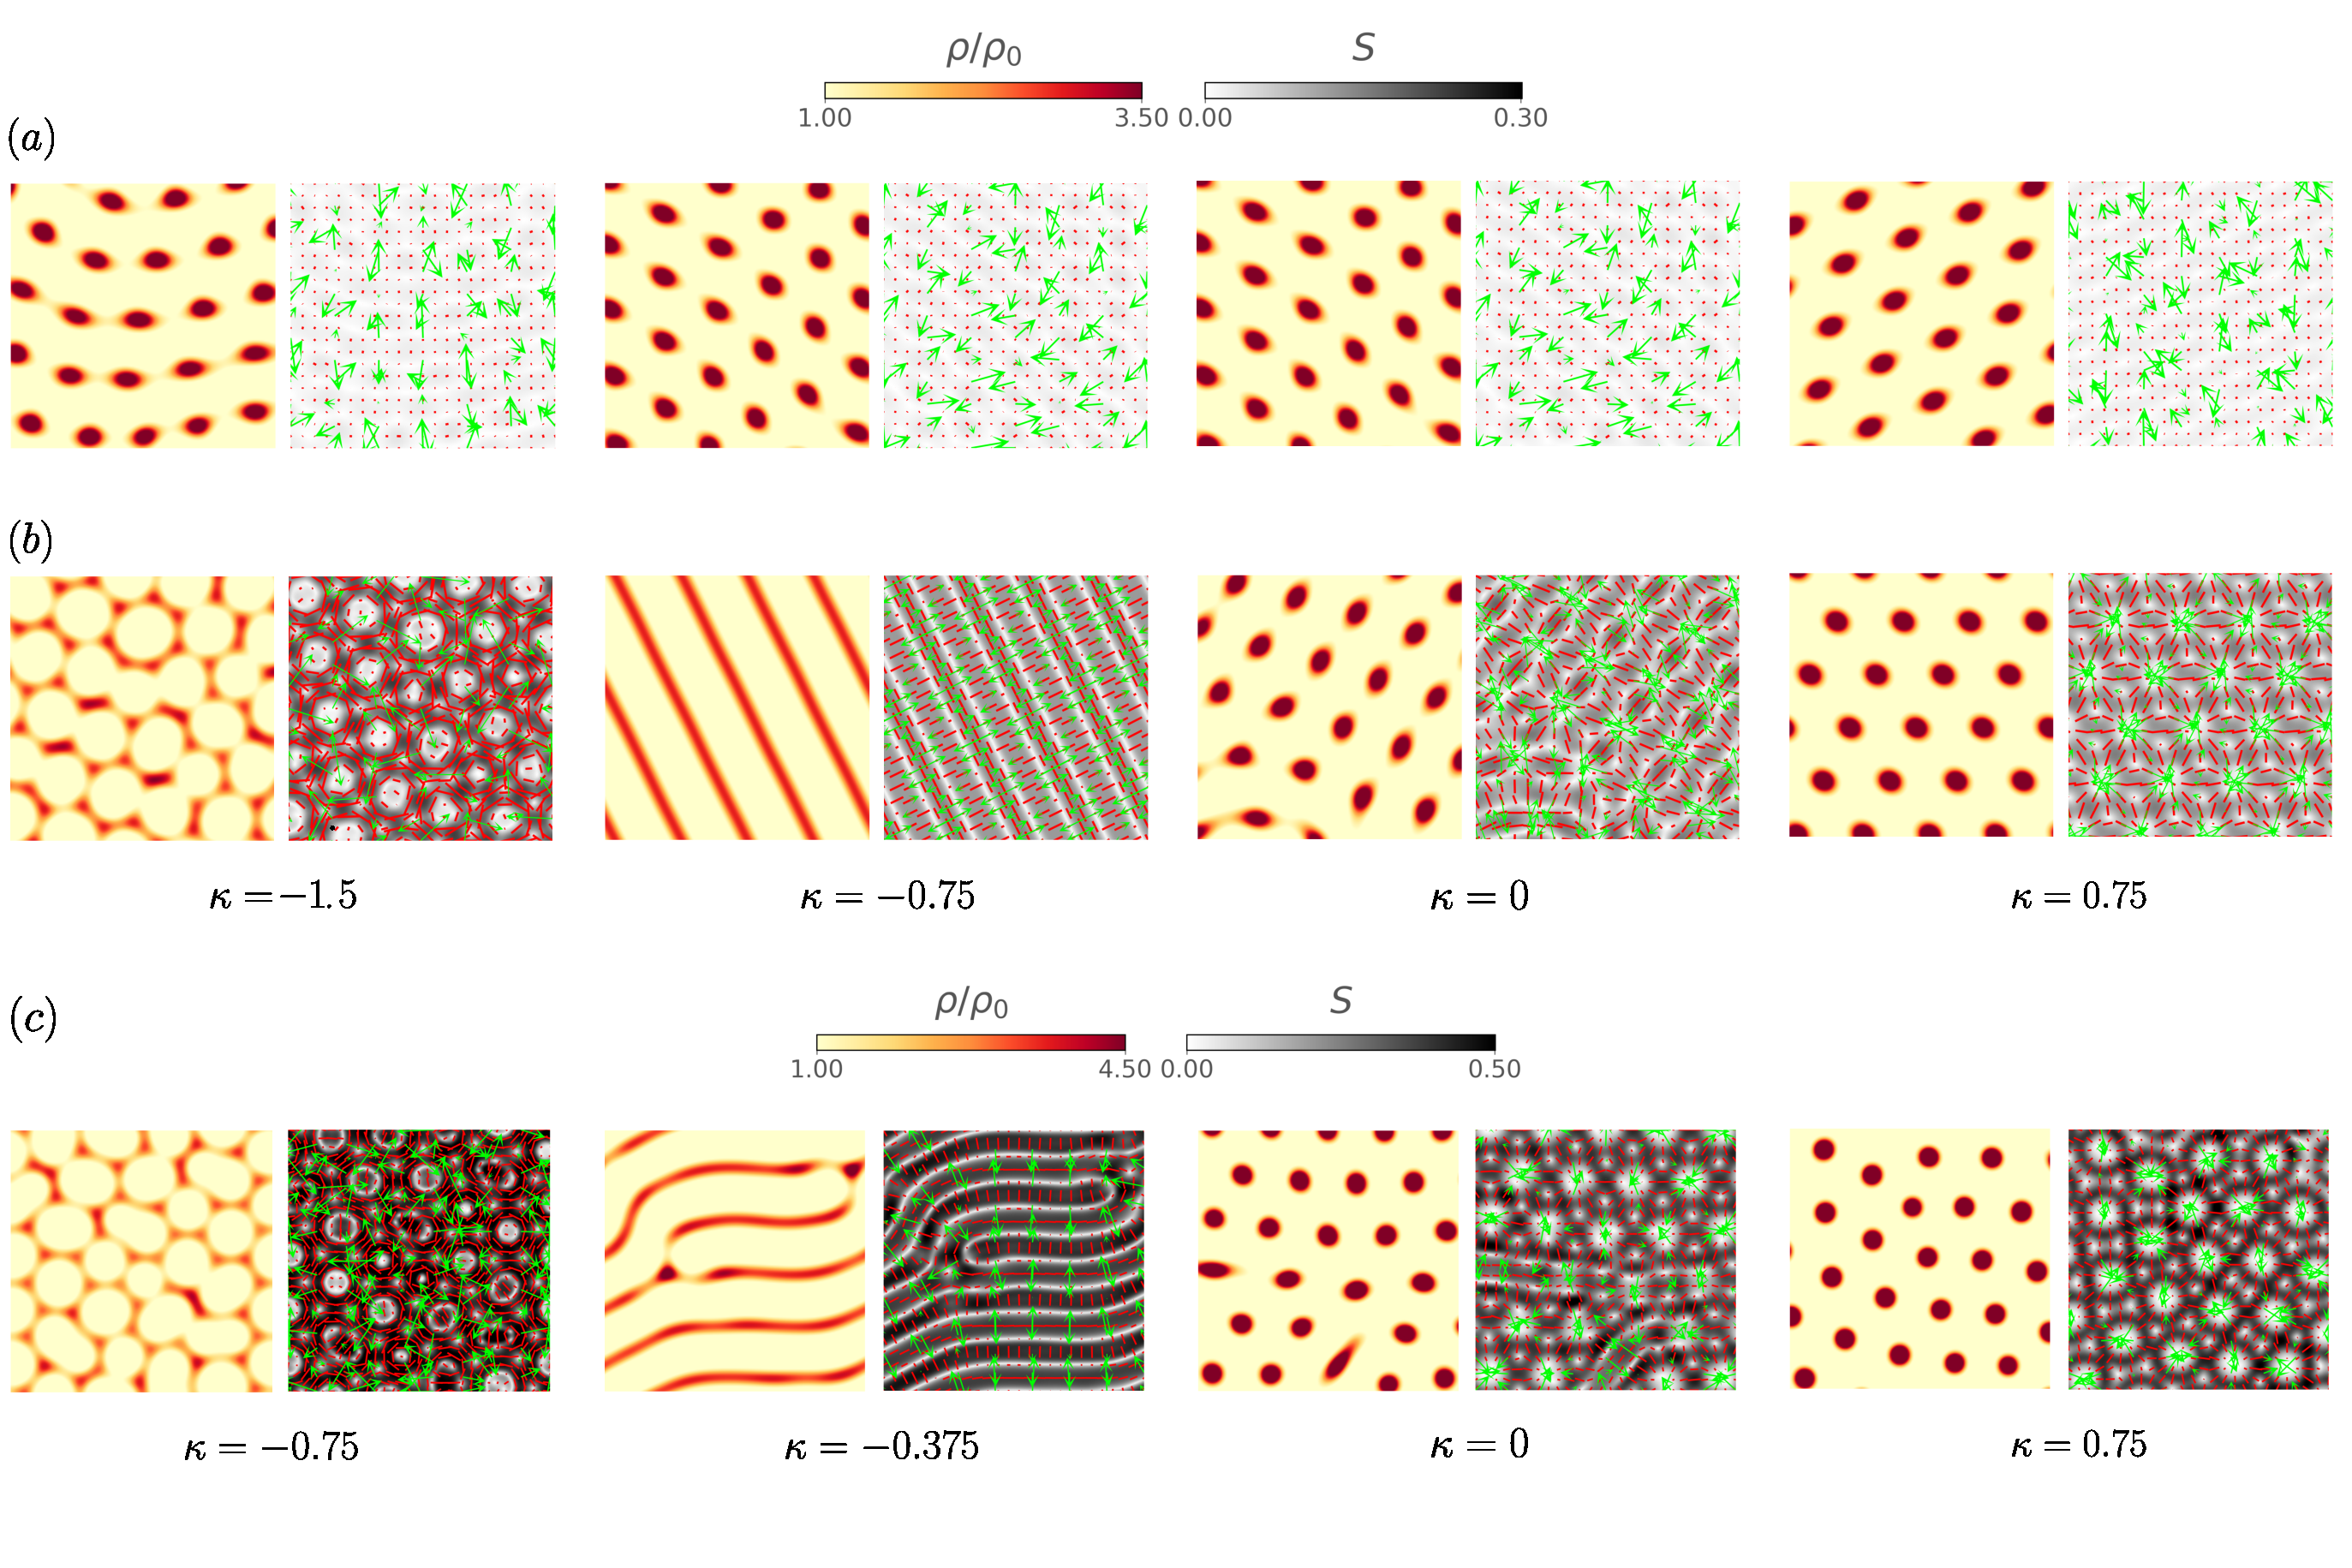
\includegraphics[width=\textwidth]{supplem_figure_1.pdf}
	\caption{\textbf{Pattern formation for a range of values of anisotropic active parameter $\kappa$ in the limit  $\lambda_{\odot} \rightarrow 0$.} (a) Pattern formation for canonical material parameters used in Fig.~\ref{fig4.2} except for  $\lambda_{\odot}=0$. (b) Here, in addition to  $\lambda_{\odot}=0$, we set $\beta^2 = 2\eta \eta_{\rm rot}$ to the largest value allowed by Onsager's inequality. (c) Using the parameters as in (b), we further increase friction as detailed in Table~\ref{defaulttable}.
	}
	\label{supplem_fig_1}
\end{figure}



\begin{figure}[p]
	\centering
	\includegraphics[width=0.95\textwidth]{supp_fig_stress.pdf}
		\caption{\textbf{Stress distribution along ($\sigma_{\vert\vert}$) and perpendicular to ($\sigma_{\perp}$) the dense nematic bundles.} The left column shows the density distribution, the middle column the total stress along and perpendicular to nematic bundles, and the right column the different contributions to the total stress dominated by  the active and the viscous components. In all cases, we consider for convenience fully nonlinear simulations in 1D to easily define the orthogonal directions relative to the self-organized pattern. (a) to (c) show patterns obtained for negative tension anisotropy $\kappa$ of increasing magnitude, whereas (d) shows a chaotic pattern resulting from a large hydrodynamic length. The modal parameters used in the plots are the same as in Figs.~\ref{fig4.2} and~\ref{fig4.3} and are described in Tables~\ref{defaulttable} and A.3. }
	\label{supplem_fig_2}
\end{figure}



\begin{figure}[p]
	\centering
	\includegraphics[width=0.65\textwidth]{supplem_figure_2.pdf}
	\caption{ \textbf{Discrete network simulations}. (I) Microstructural modeling approach using cytosim. (a) The nematic ordering of the network, $S$, measured with respect to a director $\hat{\bm{n}}$, is controlled by a system-wide restraining energy. (b) Actin filaments are represented by sets of connected particle points that are kept at a fixed distance (segmentation) and have finite bending rigidity $\kappa_A$. Crosslinkers are Hookean springs with stiffness $K_X$ and resting length $\ell_X$. Myosin motors are Hookean springs with stiffness $K_M$ and resting length $\ell_M$; their ends can `walk' on filaments at a speed $v_M$, which is affected by force application.  (II) Simulation protocol to quantify active tension anisotropy. (a) Initial fiber seeding without orientational bias. (b) Rearrangement of the network to provide a nematic orientation characterized by the ordering parameter $S_0$. (c) Introduction of anchors to measure the active forces exerted at the system's boundaries. (d) Introduction of crosslinkers and myosin motors and deactivation of the restraining potential, which drives the system out-of-equilibrium and allows us to track tensions at the boundary, (e,f). (III) Protocol to  quantifying the orientational activity parameter $\rho \lambda_{\odot}$. (a) Initial fiber seeding without orientational bias. (b) Athermal rearrangement of the network to provide a nematic orientation characterized by the ordering parameter $S_0$. (c) Estimation of the model parameter $\eta_{\rm rot}$, which characterizes the dynamics of athermal network reorientation in the presence of a restraining potential of stiffness $\mathcal{K}_S$; note that a single value of $\eta_{\rm rot}$  describes the system behavior for various $S_0$. (d) Introduction of crosslinkers and myosin motors, activation of system temperature, and deactivation of the restraining potential. The dynamics of orientational order of the system drive out-of-equilibrium are then tracked during a time period (d,e). }
	\label{supplem_fig_3}
\end{figure}

\section{Parameters used for the numerical studies}  \label{appendix_1_sec_9}
\begin{table}[H]
	\begin{tabular}{l|cccc} \textbf{Params.} &  Fig.~\ref{sec_1_chap_3_fig_1}    &  Fig.~\ref{sec_1_chap_3_fig_2}       &  Fig.~\ref{sec_1_chap_3_fig_3}      &  Fig.~\ref{sec_1_chap_3_fig_3.5}         \\ \hline 
		$\rho_0$ [\si{\micro \meter}]  & 0.2 & 0.2 & \textemdash & \textemdash  \\ 
		$\eta$ [\si{\pascal \second}] & $10^4$ & $10^4$ & $10^4$ & $10^4$  \\ 
		$\ell_s = \sqrt{\eta/\gamma}$ [\si{\micro \meter]} &10 &10&10 &10 \\
		$k_d$ [\si{\second}$^{-1}$] &0.1 & 0.1 & \textemdash & \textemdash\\
		$D$ [\si{\micro \meter}$^2$ s$^{-1}$] & 0.02& 0.02 & \textemdash & \textemdash \\
		$\eta_{\rm rot} / \eta$ & 1&1 & 1&1\\
		$\beta / \eta$ & -1 & -1,-0.1 & -0.2 & -0.2 \\
		$a/\eta$ $[\si{\second}^{-1}]$ & 1 &1  & -1 &-1 \\
		$b/\eta$ $[\si{\second}^{-1}]$  &4 &4  & 2 &2  \\
		$L/\eta$ $[\si{\micro \meter}^2  \si{\second}^{-1}$] & $ 0.01$&$ 0.01$ & [$8 \times 10^{-4}$ ,$0.18  $ ] & $8 \times 10^{-4}$  \\
		$\rho_0 \lambda_{\bigodot}^0 /(2a)$ &0.4  &0.2,0.4,0.6  & \textemdash & \textemdash  \\
		$\lambda^0/\eta \, [\si{\second}^{-1}]$ &0.12& 0.12  &\textemdash & \textemdash\\
		$\delta \lambda/ \lambda$   & 5& 5 &  \textemdash &  \textemdash\\
		$\kappa = \lambda_{\rm aniso}/\lambda$  & [0.5,2]  &1.0 & \textemdash &\textemdash,     \\
		$\lambda_{\rm aniso}/\eta [s^{-1}]$  & \textup{see value of} $\kappa$  &\textup{see value of} $\kappa$  & 0 &$8.9 \times 10^{-3}$, $0.036$,$0.08$,$0.32$     \\
		$\ell_0 $  [\si{\micro \meter}]  & 20  & 20 & 1  & 1 \\
		$\ell_a = \sqrt{L/\left(\lambda_{\rm aniso}S_0\right)}$   & \textemdash  & \textemdash & $\infty$  & $\infty, 0.3,0.15,0.1,0.05,0.04$ \\
		$$ [\si{\micro \meter}] & &  &   &  \\
		$\ell_p = \sqrt{L/(2|a|-\rho_0\lambda_{\odot})}$   & 0.056 &  0.0527,0.056,0.06   & [0.02, 0.3]  & 0.02 \\
		$$ [\si{\micro \meter}] & &  &   &  \\
		\hline 
	\end{tabular}
	\caption{Overview of parameters used for numerical studies of Chapter~\ref{chap_3}.}
	\label{modal_parameters}
	\end{table}

	\begin{table}[hb]
	\begin{center}\begin{tabular}{l|ccccc} Parameters & Fig.~\ref{fig4.2} & Fig.~\ref{supplem_fig_1}(a) & Fig.~\ref{supplem_fig_1}(b) & Fig.~\ref{supplem_fig_1}(c)     \\ \hline \\
			$\bar{k}_d$  &  0.1& 0.1 &0.1&0.01  \\
			$\bar{L}$  & 1 & 1 &1&1   \\
			$\bar{c}_0$  & 4&  4&4 &0.4 \\
			$\bar{b}$  & 20& 20&20&2\\
			$\bar{\eta}_{\rm rot}$  &  1&  1& 1&1 \\
			$\bar{\beta}$  &  -0.2&  -0.2&-$\sqrt{2}$&-$\sqrt{2}$  \\
			$\bar{\lambda}_\odot$ &  6& 0 &0&0  \\
			$\bar{\lambda}$ &$1.3 \bar{\lambda}_{\rm crit}$  & $1.3 \bar{\lambda}_{\rm crit}$&$1.3 \bar{\lambda}_{\rm crit}$&$1.3 \bar{\lambda}_{\rm crit}$  \\
			$\kappa$ & [-0.8,0.8] & [-1.5,-0.75,0,0.75]&[-1.5,-0.75,0,0.75]&[-0.75,-0.375,0,0.75]  \\
			$\ell_0$ & 8 & 8 &8&8  \\
			\hline
		\end{tabular}
	\end{center}
	\caption{Model parameters used in figures  of Chapter~\ref{chap_4}.}
	\label{defaulttable}
    \end{table}

	\begin{sidewaystable}
	\begin{minipage}[c][\textheight][c]{\textwidth}
		\begin{center}
			\begin{tabular}{l|cccccccccccc} Params.& 4.1 &  4.2 & 4.3(I,II) & 4.3(III,IV) & 4.4 & 4.5a(III) & 4.5b(II,III) & 4.5b(I)& 4.5a(II) \\ \hline \\
				$\bar{k}_d$  &0.01&0.1&  0.1& 0.1 &0.1&0.1&10,20&20& 0.1  \\
				$\bar{L}$  &1&1& 1 &1& 1 &1& 1 & 1& 1\\
				$\bar{c}_0$ &0.4&4 &  4& 4& 4& 4&4 &200&-0.05\\
				$\bar{b}$  &2&20& 20& 20&20& 20&20&4000&20\\
				$\bar{\eta}_{\rm rot}$ &0& 1&1 1&&  1&  1&1&1&1  \\
				$\bar{\beta}$ & 0&-0.2& -0.2,0 & -$\sqrt{2}$,-0.2&-0.2&-0.2&-0.2 &-0.2&-0.2 \\
				$\bar{\lambda}_\odot$ &0&6&  6& 6 &6&6&6&1800&10.05\\
				$\bar{\lambda}$ &1.3$\bar{\lambda}_{\rm crit}$&1.3$\bar{\lambda}_{\rm crit}$&1.3$\bar{\lambda}_{\rm crit}$  & 1.3$\bar{\lambda}_{\rm crit}$ & 1.3$\bar{\lambda}_{\rm crit}$& Same as Movie~4.1 & 1.3$\bar{\lambda}_{\rm crit}$&1.3$\bar{\lambda}_{\rm crit}$&1.3$\bar{\lambda}_{\rm crit}$  \\
				$\kappa$ &0&-0.2,0.05,0.7& -0.2 & 0.2&-0.2,-0.5,-0.8  &-0.2&-0.2&-0.2&-0.2\\
				$\ell_0$ &8&8&8 & 8 &8&Same as Movie~4.1&8 &8&8  \\
							\hline
			\end{tabular}
		\end{center}
				\caption{Model parameters used in movies of Chapter~\ref{chap_4}. Below the first column consist of the model parameters and the rest of the columns labeled as $4.$x corresponds to the movie number. The caption of each video is described in the Appendix~\ref{appendix_3}.}
						\label{supplem_table_2}
	\end{minipage}
\end{sidewaystable}

\begin{sidewaystable}
	\begin{minipage}[c][\textheight][c]{\textwidth}
		\begin{center}\begin{tabular}{lccccc} \multicolumn{2}{l}{\textbf{Reference}}  &  Geometry and size [ \si{\micro\meter}\textbf{ ]} & $kT$ \textbf{[ }\si{\pico\newton \micro\meter}\textbf{ ]} & Time step [ \si{\second}\textbf{ ]} & $\nu$ \textbf{[ }\si{\pascal \second}\textbf{ ]} \\ \hline \\
				
				\multicolumn{2}{l}{Present work}  & Square: $\ell = 5$ & 0 or 0.0042 & 0.005 & 1  \\
				
				\multirow{3}{*}{\cite{Cortes2020}} & MM1 & Rectangle: 2 $\times$ 0.2 & 0.0042 & 0.001 & 1 \\
				
				& MM4 & Rectangle: 9.424 $\times$ 1 & 0.0042 & 0.001 & 1 \\
				
				& MM3 \& MM5 & Circle: $R = 1.5$ & 0.0042 & 0.001 & 1 \\
				
				\multicolumn{2}{l}{Cortex simulations in  \cite{Wollrab2019}} & Square: $L = 8$ & 0.0042 & 0.002 & 0.18 \\
				
				\multicolumn{2}{l}{ \cite{Bun2018}} & Circle: $R = 10$ & 0.0042 & 0.01 or 0.1 & 0.3  \\
				
				\multicolumn{2}{l}{Model with turnover in  \cite{Belmonte2017}} & Square: $L = 16$ & 0.0042 & 0.001 & 0.1 \\
				
				\multicolumn{2}{l}{ \cite{Descovich2017}} & Circle: $R = 15$ & 0.0042 & 0.002 & 1 \\
				
				\multicolumn{2}{l}{\cite{Ding2017}} & Circle: $R = 10$ & 0.0042 & 0.001 & 0.1 \\
				
				\multicolumn{2}{l}{\cite{Ennomani2016}} & Ring: $R = 4.5$, $t \approx 0.5 $ & 0.0042 & 0.01 & 0.18 \\
				
			\end{tabular}
		\end{center}
			\caption{Global parameters adopted in this study and in previous microstructural models that used cytosim.}
		\label{tab:GlobalParamTable}
	\end{minipage}
\end{sidewaystable}

\begin{sidewaystable}
	\begin{minipage}[c][\textheight][c]{\textwidth}

		\begin{center}
			\begin{tabular}{lcccccc} \multicolumn{2}{l}{\textbf{Reference}} & $\ell_A$ \textbf{[ }\si{\micro\meter}\textbf{ ]} & $\rho_A$ \textbf{[ }\si{\micro\meter/\micro\meter}$^{2}$\textbf{ ]} & $s_A$ \textbf{[ }\si{\micro\meter}\textbf{ ]} & $\kappa_A$ \textbf{[ }\si{\pico\newton \micro\meter}$^{2}$\textbf{ ]} & $r_A$ \textbf{[ }\si{\%/\second}\textbf{ ]} \\ \hline \\
				
				\multicolumn{2}{l}{Present work}  & 1.3 & 78, 156, or 234 & 0.2 & 0.1 & 20  \\
				
				\multirow{4}{*}{Ref. \cite{Cortes2020}} & MM1 & 2 & 1800 & $0.05 - 0.1$ & 0.06 & 0 \\
				
				& MM3 & $1.3 \pm 0.3$ & $50.9 - 81.5$ & $0.05 - 0.1$ & 0.06 & 0 \\
				
				& MM4 & $1.3 \pm 0.3$ &  $38.2 - 61.1$ & $0.05 - 0.1$ & 0.06 & 0 \\
				
				& MM5 & $1.3 \pm 0.3$ &  $50.9 - 81.5$ & $0.05 - 0.1$ & 0.06 & 0 \\
				
				\multicolumn{2}{l}{Cortex simulations in Ref. \cite{Wollrab2019}} & $0.1 - 4.0$ & $5.5 - 218.8$ & $0.1 - 0.4$ & 0.075 & 0 \\
				
				\multicolumn{2}{l}{Ref. \cite{Bun2018}} & 1.5 & 23.9 & 0.15 & 0.07 & 0  \\
				
				\multicolumn{2}{l}{Model with turnover in Ref. \cite{Belmonte2017}} & 5 & 27.3 & $0.1 - 0.2$ & 0.075 & $1.1 - 18.3$ \\
				
				\multicolumn{2}{l}{Ref. \cite{Descovich2017}} & $1.3 \pm 0.3$ & $3.4 - 5.4$ & 0.1 & 0.06 & 0 \\
				
				\multicolumn{2}{l}{Ref. \cite{Ding2017}} & $2.2$ & 35 & \textemdash & 0.05 & 0 \\
				
				\multicolumn{2}{l}{Ref. \cite{Ennomani2016}} & $0.95 - 1.75$ & $117.2 - 154.2$ & \textemdash & $0.042 - 0.063$ & 0 \\
				
			\end{tabular}
		\end{center}
			\caption{Actin filament parameters adopted in this study and in previous microstructural models that used cytosim.}
		\label{tab:ActinParamTable}
	\end{minipage}
\end{sidewaystable}

	\begin{sidewaystable}
	\begin{minipage}[c][\textheight][c]{\textwidth}
		\begin{center}\begin{tabular}{lcccccccccc}
				\multicolumn{2}{l}{\multirow{2}{*}{\textbf{Reference}}} & $\rho_M$ & $K_M$ & $\ell_M$ & $r_M^b$ & $d_M^b$ & $r_M^{u,0}$ & $f_M^u$ & $f_M^{\rm stall}$ & $v_M^{\rm max}$ \\
				
				\multicolumn{2}{l}{}  &  \textbf{[ }\si{1/\micro\meter} actin\textbf{ ]} & \textbf{[ }\si{\pico\newton/\micro\meter}\textbf{ ]} & \textbf{[ }\si{\micro\meter}\textbf{ ]} & \textbf{[ }\si{1/\s}\textbf{ ]} & \textbf{[ }\si{\micro\meter}\textbf{ ]} & \textbf{[ }\si{1/\second}\textbf{ ]} & \textbf{[ }\si{\pico\newton}\textbf{ ]} & \textbf{[ }\si{\pico\newton}\textbf{ ]} & \textbf{[ }\si{\micro\meter/\second}\textbf{ ]} \\ \hline \\
				
				\multicolumn{2}{l}{Present work}  & 0.8 & 250 & 0 & 50 & 0.02 & 50 & $\infty$ & 6 & 0.3 \\
				
				\multirow{2}{*}{\cite{Cortes2020}} &  & 0.5 & 100 & 0.3 & $0.2 - 3.6$ & $0.06 - 0.12$ & $0.8 - 1.71$ & 5 & $3.85 - 15$ & $0.137 - 0.6$ \\
				
				&& $0.6 - 1.0$ & 100 & 0.3 & $0.2 - 3.6$ & $0.06 - 0.12$ & $0.8 - 1.71$ & 5 & $3.85 - 15$ & $0.137 - 0.6$ \\
				
				\multicolumn{2}{l}{Cortex simulations} & $2 - 64$ & 100 & 0 & 10 & 0.01 & 0.5 & $\infty$ & 4 & 2  \\
					
	\multicolumn{2}{l}{ \cite{Wollrab2019}} &  &  &  &  &  &  &  &  &   \\			
				\multicolumn{2}{l}{Ref. \cite{Bun2018}} & 2.7 & 250 & 0.01 & 10 & 0.01 & 0.1 & 3 & 6 & 0.02 \\
				
				\multicolumn{2}{l}{Model with turnover } & 3.2 & 500 & 0 & 10 & 0.01 & 0.3 & $\infty$ & 6 & 0.2 \\
				\multicolumn{2}{l}{\cite{Belmonte2017}} & &  &  &  & & &  &  & \\				
				\multicolumn{2}{l}{\cite{Descovich2017}} & $0.5 - 0.8$ & 1'400 & 0.32 & 0.2 & 0.33 & 0.3 & 3.85 & 24.5 & 0.1 \\
				
				\multicolumn{2}{l}{\cite{Ding2017}} & 0 or 5.8 & 250 & 0 & 10 & 0.01 & 0.5 & $\infty$ & 6 & 0.5 \\
				
				\multicolumn{2}{l}{\cite{Ennomani2016}} & $0.3 - 0.4$ & 100 & 0.03 & 5 & 0.05 & 0 & 3.65 & 2 & 0.3 \\
				
			\end{tabular}
		\end{center}
			\caption{Myosin motor parameters adopted in this study and in previous microstructural models that used cytosim.}
		\label{tab:MotorParamTable}
	\end{minipage}
\end{sidewaystable}

\hspace{1cm}





	
	
